\section{Ontology details}

The power grid ontology is aimed to give a basis for representing power grids in terms of power production, consumption and transmission. For that purpose the following classes, as listed in figure \ref{fig:classes} were designed.
The most basic building blocks are the \textit{NetworkEntities} which model all physical entities 
a network may consist of and are disjoint. There are \textit{Producers} adding power to the network, \textit{Consumers} drawing energy from the network, \textit{TransportEntities} transporting the energy between exactly two other network entities and \textit{Transformers} managing splits, merges and changes in the transmission type of \textit{TransportEntities}. \\
Those transmission types are modelled in the \textit{TransmissionType} class. This class is divided into two disjoint subclasses \textit{ACTransmission} for alternating current and \textit{DCTransmission} for direct current. \\
Each \textit{TransportEntity} furthermore has a \textit{CableType} indicating the layout of a power line. There are 3 disjoint alternatives: regular \textit{TransmissionLines}, \textit{UndergroundCables} and \textit{UnderseaCables}. \\
Finally every \textit{NetworkEntity} is part of a specific \textit{Network}.

\begin{figure}
\centering
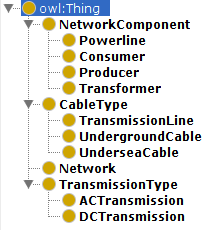
\includegraphics[scale=.75]{img/classes.png} 
\label{fig:classes}
\caption{Class hierarchy of the Power Grid ontology.}
\end{figure}